\documentclass{standalone}
\usepackage{tikz}
\usetikzlibrary[arrows,positioning,matrix]

\begin{document}
\begin{tikzpicture}
  \node[draw=none] (example) {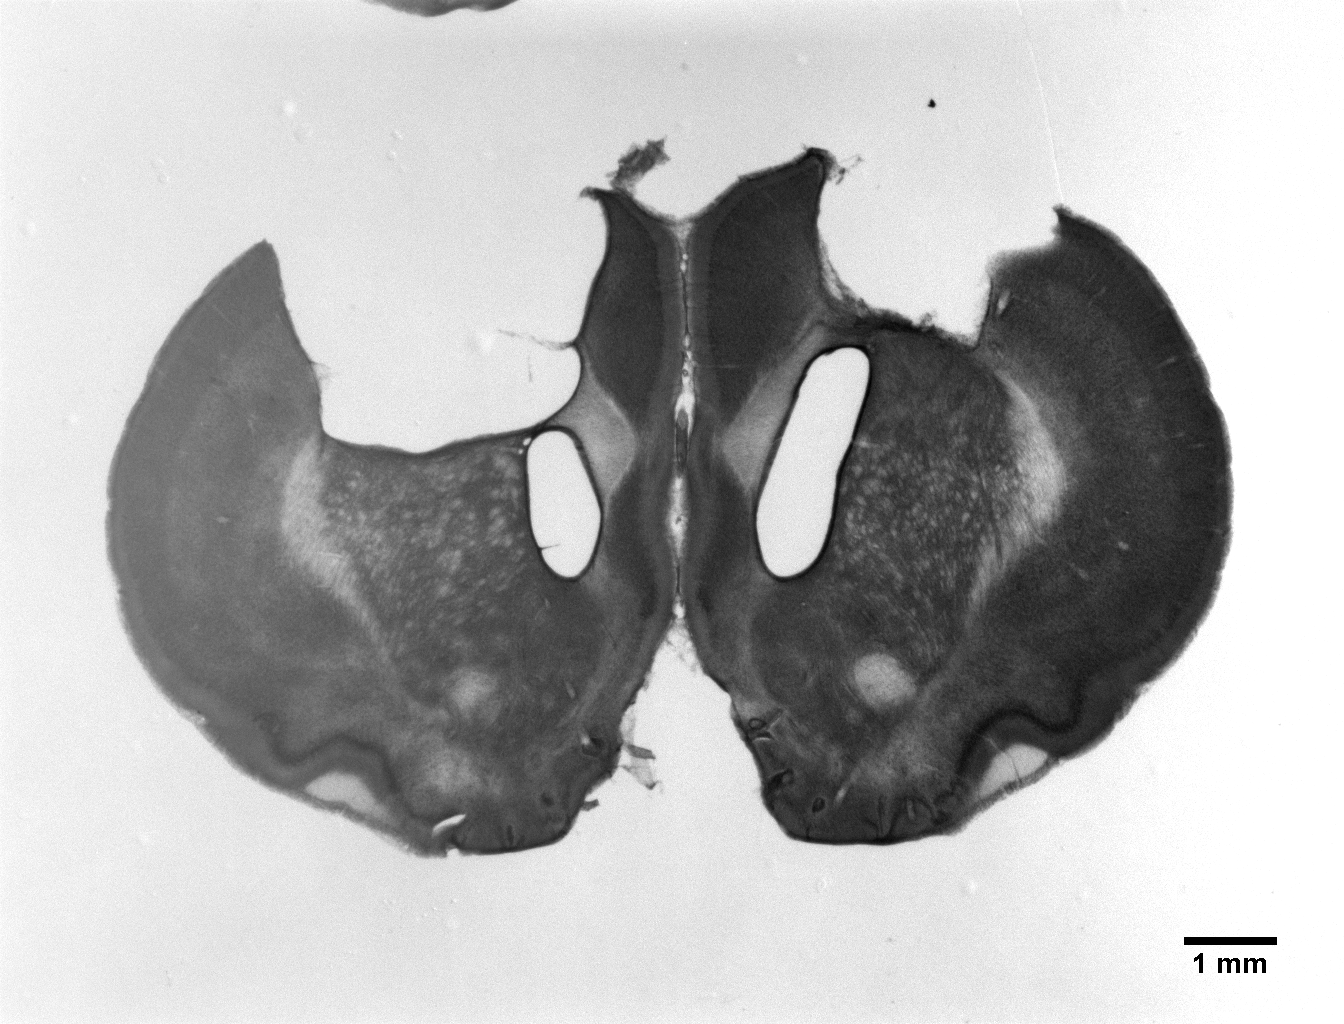
\includegraphics[width=0.5\textwidth]{elements/extendedlesionB_viewplate_bregma2mm-slice32}};
  \node[draw=none,above left=1.5mm and -4mm of example] {A};
  
  \node[draw=none,right=1mm of example] (schematic) {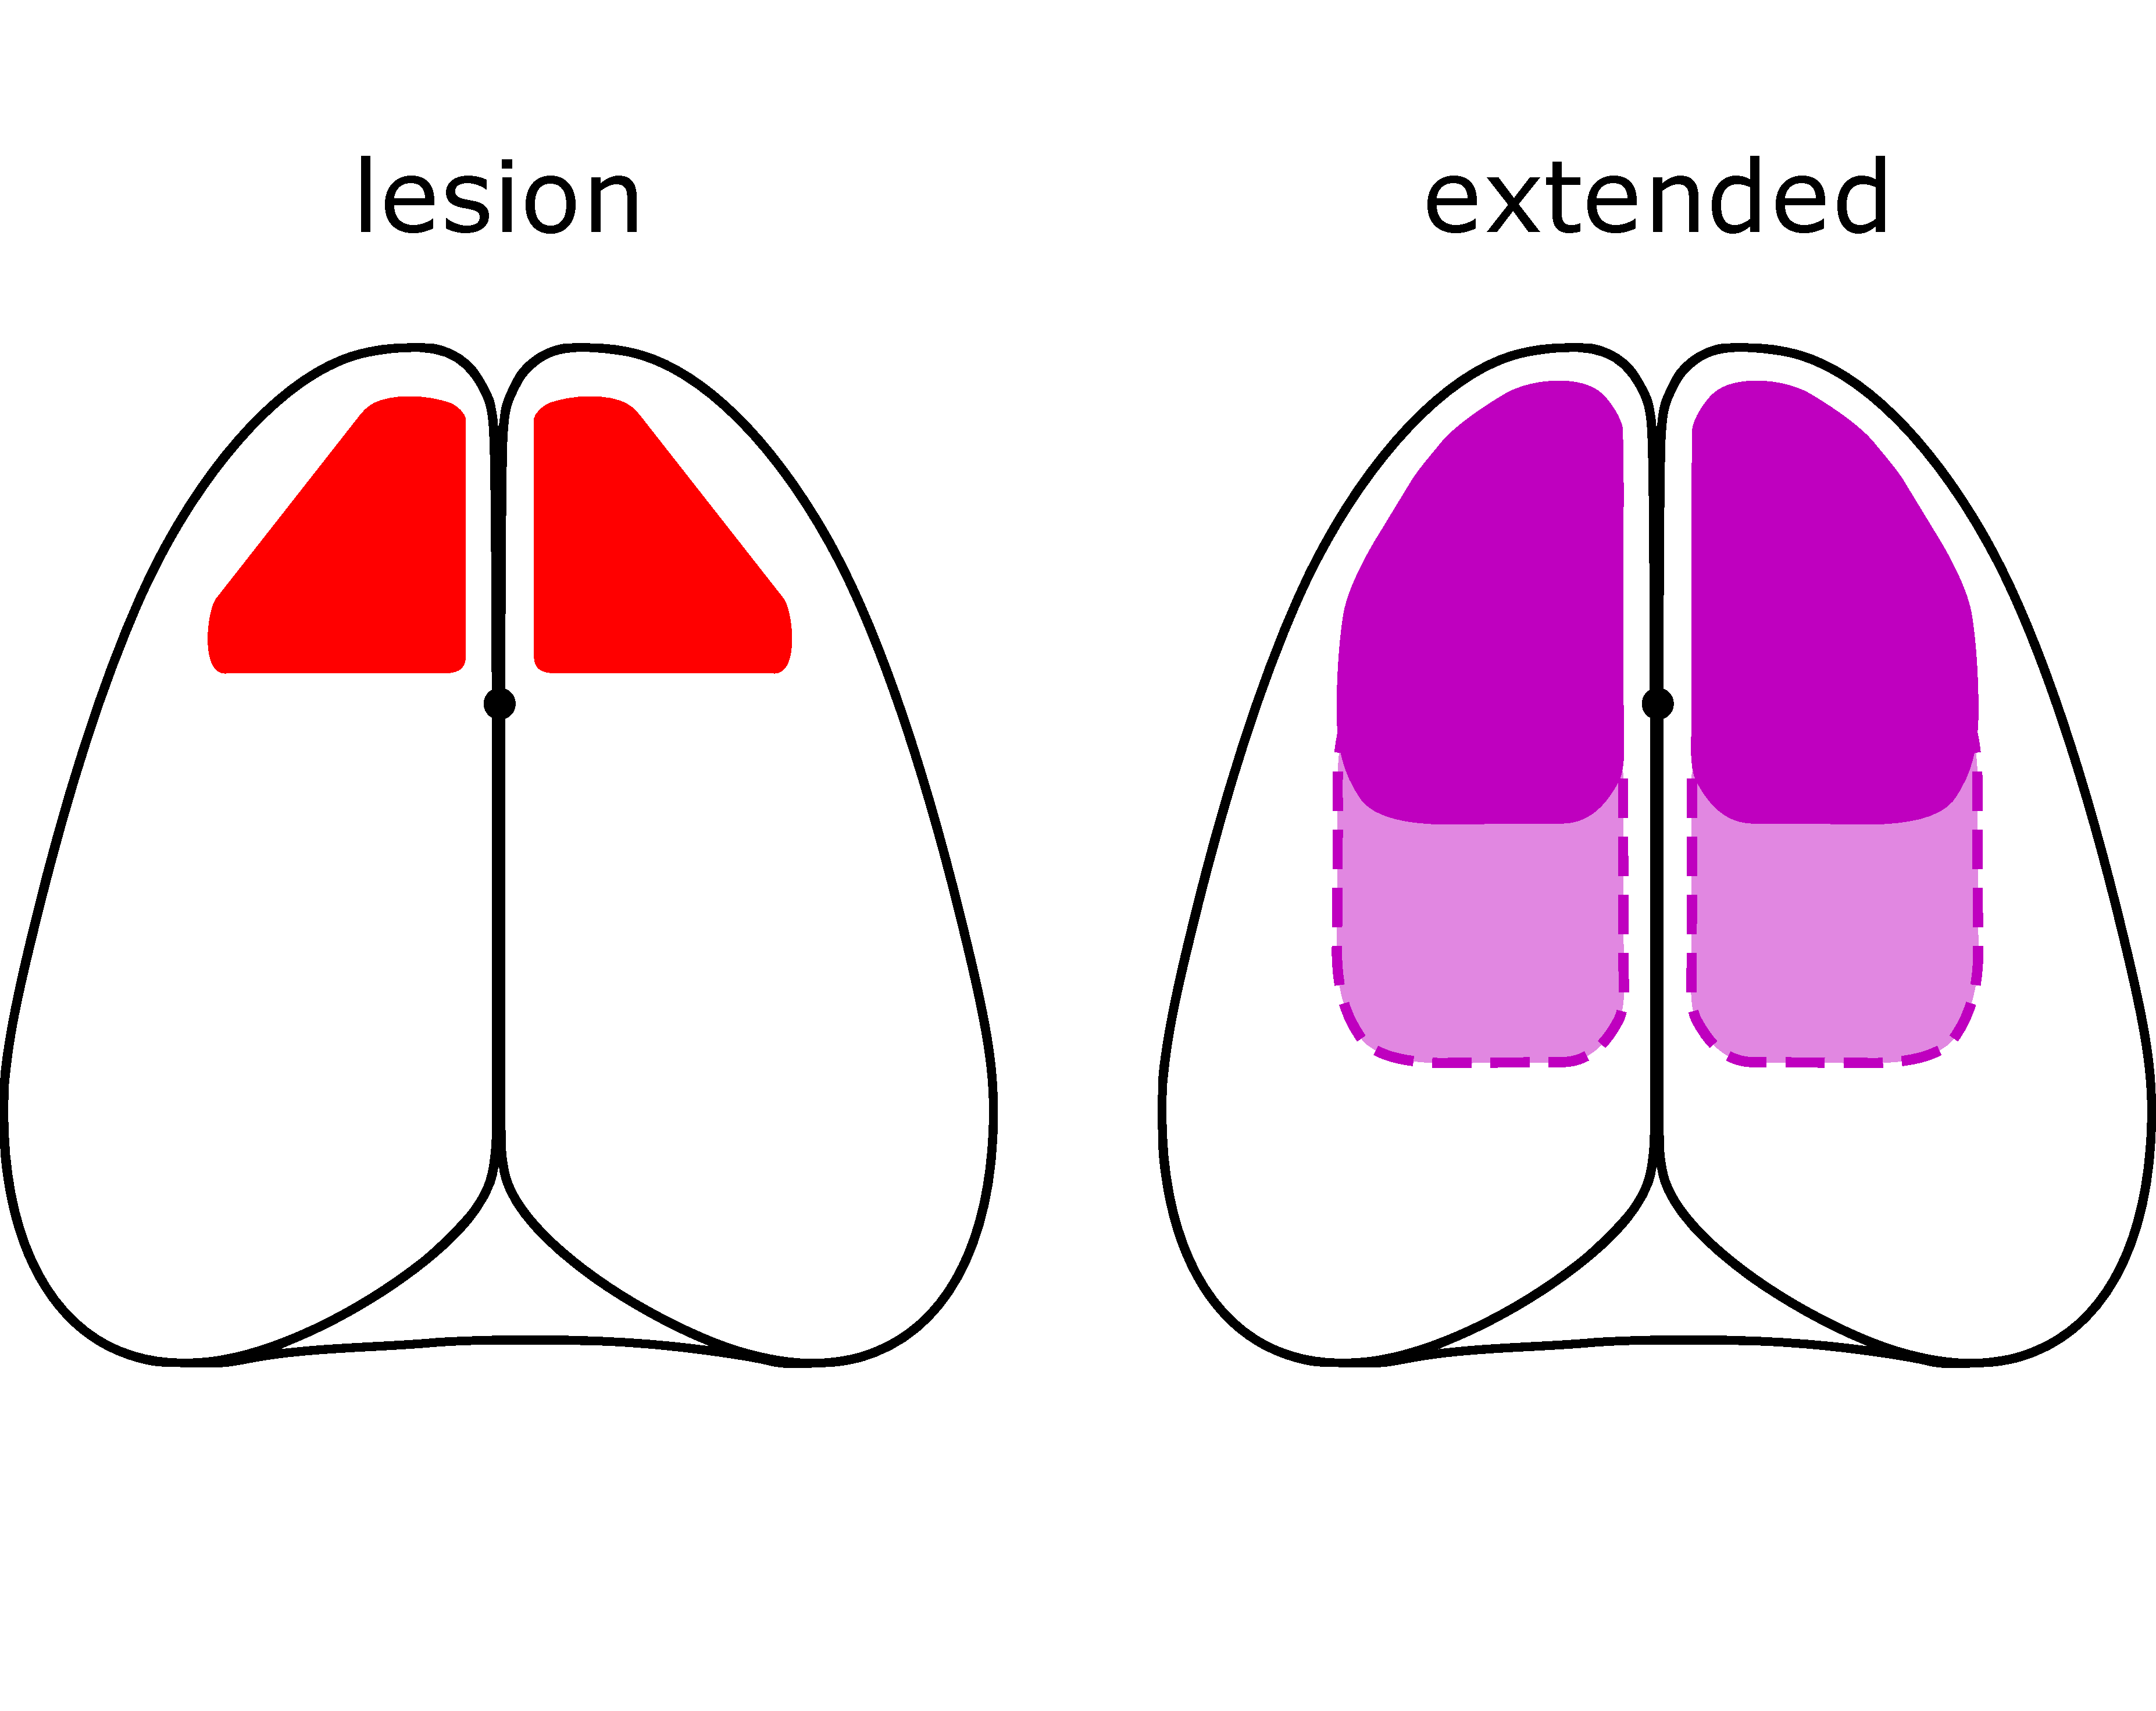
\includegraphics[width=0.5\textwidth]{elements/extendedlesions}};
  \node[draw=none,above left=0.6mm and -4mm of schematic] {B};
\end{tikzpicture}
\end{document}